\documentclass{article}
    % General document formatting
    \usepackage[margin=0.7in]{geometry}
    \usepackage[parfill]{parskip}
    \usepackage[utf8]{inputenc}
    \usepackage{amsmath}
    \usepackage{amssymb}
    \usepackage{tikz}
    \usepackage{fancyhdr}
    \usepackage{listings}

\pagestyle{fancy}
\fancyhf{}
\rhead{Edgar Jacob Rivera Rios - A01184125}

\begin{document}
\begin{titlepage}

    \newcommand{\HRule}{\rule{\linewidth}{0.5mm}} % Defines a new command for the horizontal lines, change thickness here

    \center % Center everything on the page

    %----------------------------------------------------------------------------------------
    %	HEADING SECTIONS
    %----------------------------------------------------------------------------------------

    \textsc{\LARGE Tecnológico de Monterrey}\\[1.5cm] % Name of your university/college
    \textsc{\Large Fundamentos de computación}\\[0.5cm] % Major heading such as course name
    %\textsc{\large Minor Heading}\\[0.5cm] % Minor heading such as course title

    %----------------------------------------------------------------------------------------
    %	TITLE SECTION
    %----------------------------------------------------------------------------------------

    \HRule \\[0.4cm]
    { \huge \bfseries Homework 6}\\[0.4cm] % Title of your document
    \HRule \\[1.5cm]

    %----------------------------------------------------------------------------------------
    %	AUTHOR SECTION
    %----------------------------------------------------------------------------------------

    \begin{minipage}{0.4\textwidth}
    \begin{flushleft} \large
    \emph{Student:}\\
    Jacob \textsc{Rivera} % Your name
    \end{flushleft}
    \end{minipage}
    ~
    \begin{minipage}{0.4\textwidth}
    \begin{flushright} \large
    \emph{Professor:} \\
    Dr. Hugo \textsc{Terashima} % Supervisor's Name
    \end{flushright}
    \end{minipage}\\[2cm]

    % If you don't want a supervisor, uncomment the two lines below and remove the section above
    %\Large \emph{Author:}\\
    %John \textsc{Smith}\\[3cm] % Your name

    %----------------------------------------------------------------------------------------
    %	DATE SECTION
    %----------------------------------------------------------------------------------------

    {\large \today}\\[2cm] % Date, change the \today to a set date if you want to be precise

    %----------------------------------------------------------------------------------------
    %	LOGO SECTION
    %----------------------------------------------------------------------------------------

    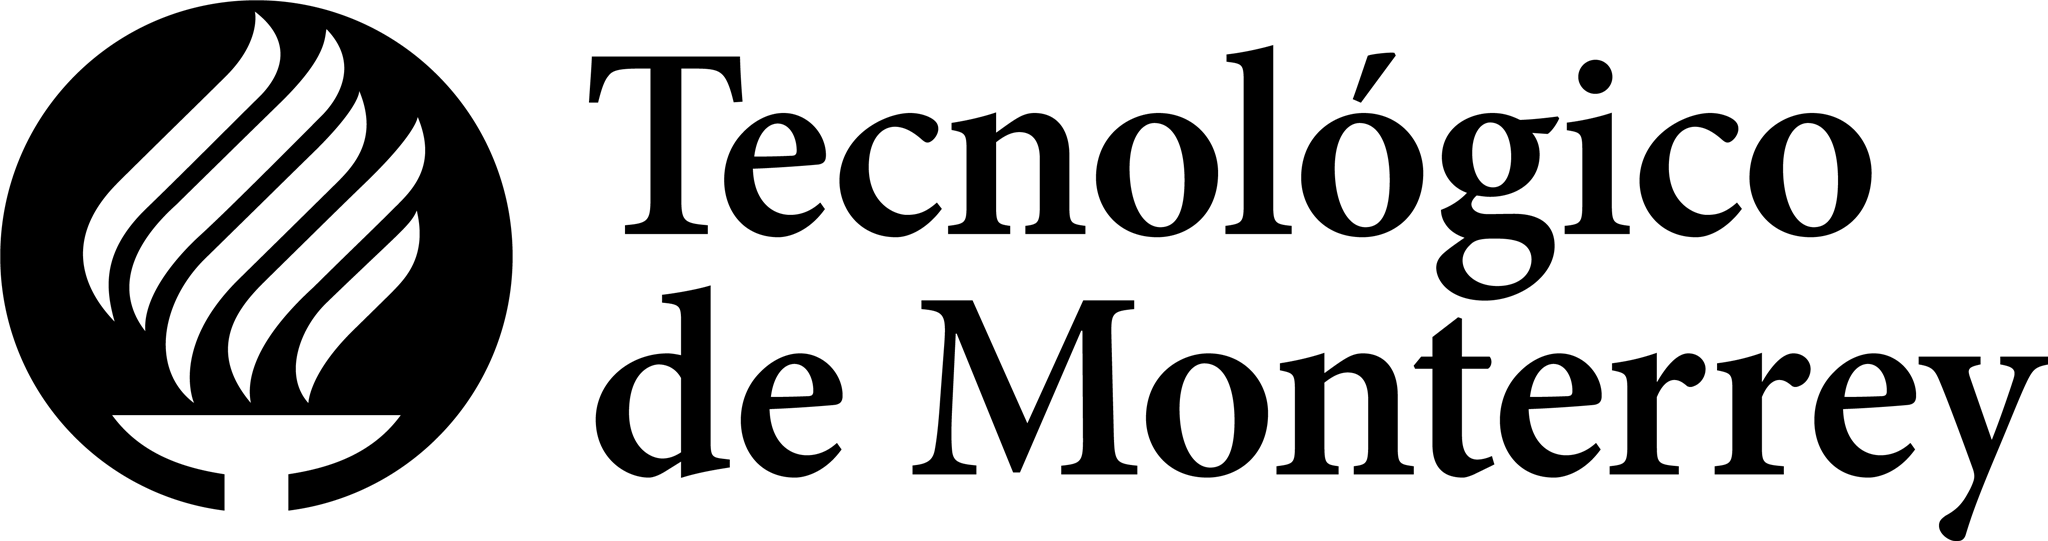
\includegraphics[width=0.4\textwidth,height=\textheight,keepaspectratio]{logo-tec-negro.png} % Include a department/university logo - this will require the graphicx package

    %----------------------------------------------------------------------------------------

    \vfill % Fill the rest of the page with whitespace

\end{titlepage}


\section{Problems}
Solve the following problems:
\begin{enumerate}
    \item For the selection algorithm, analyze and discuss the resulting complexity when the initial list is divided into groups of 19 elements (instead of 15). Derive the proper conclusions.

    \item Given  a  set  of $n$ numbers,  we  want  to  find  the $i$ largest  in  sorted  order  using  a  comparison-based algorithm. Analyze and compare the following methods in terms of $n$ and $i$:
    \begin{enumerate}
        \item Sort the numbers, and list the $i$ largest.
        \item Build a max-priority queue (like a heap) with the numbers and extract the minimum $i$ items.
        \item Use the k-max (session 06) to find the $i$-th largest, partition around that number, and sort the $i$ largest.
    \end{enumerate}

    \item For $n$ distinct elements $x_1, x_2, ..., x_n$ with positive weights $w_1, w_2, ..., w_n$ such that $\sum^{n}_{i=1} w_i= 1$, the weighted (lower) median is the element $x_k$ satisfying $\sum_{x_i<x_k}w_i < \frac{1}{2}$ and $\sum_{x_i>x_k}w_i \leq \frac{1}{2}$

    For example, if the elements are 0.1, 0.35, 0.05, 0.1, 0.15, 0.05, 0.2 and each element equals its weight then the median is 0.1, but the weighted median is 0.2.
    \begin{enumerate}
        \item Argue that the median of $x_1, x_2, ..., x_n$ is the weighted median of the $x_i$ with weights $w_i= 1/n$ for $i= 1,2, ..., n$
        \item Show how to compute the weighted median ofnelements inO(nlogn) worst-case using sorting.
        \item Show how to compute the weighted median ofnelements inO(n) worst-case.
    \end{enumerate}

    \item Investigate  on  how  the  adversary  argument  concept  can  be  used  to  determine  the  lower  bound  of merging two ordered lists.
\end{enumerate}
\end{document}